%% uis-example.tex
%% Copyright 2019-2020 N. M. Streethran (nmstreethran at gmail dot com)
%% License: GNU General Public License, Version 3 (GPL-3.0)

%%%%%%%%%%%%%%%%%%%%%%%%%%%%%%%%%%%%%%%%%%%%%%%%%
% set custom aspect ratio and import svgnames colours
\documentclass[aspectratio=169,xcolor={svgnames}]{beamer}

%%%%%%%%%%%%%%%%%%%%%%%%%%%%%%%%%%%%%%%%%%%%%%%%%
% define title, subtitle, author's name, institute, and
% date (and/or event name)
% short versions in [brackets]
% optionally define the author's email address in the \author field
% use \today to display today's date in MMM dd, YYYY format
\title[Prime Numbers]{There Is No Largest Prime Number}
\subtitle[\textit{reductio ad absurdum}]
  {The proof uses \textit{reductio ad absurdum}.}
\author[Euclid of Alexandria]{Euclid of Alexandria
  \href{mailto:euclid@alexandria.edu}{\texttt{<euclid@alexandria.edu>}}}
\institute[Musaeum]{Musaeum of Alexandria}
\date[ISPN \the\year]{27th International Symposium of Prime Numbers; \today}
% PDF metadata - optional subject and comma-separated keywords
% leave the braces blank if not applicable
\def\keywords{presentation, beamer, latex, prime numbers}
\def\subject{Presented at ISPN \the\year. License: CC BY 4.0.}

%%%%%%%%%%%%%%%%%%%%%%%%%%%%%%%%%%%%%%%%%%%%%%%%%
% import theme
\usetheme{uis}

% import bibliography file
\addbibresource{sample.bib}

% for generating dummy text
\usepackage{lipsum}

%%%%%%%%%%%%%%%%%%%%%%%%%%%%%%%%%%%%%%%%%%%%%%%%%
\begin{document}

%%%%%%%%%%%%%%%%%%%%%%%%%%%%%%%%%%%%%%%%%%%%%%%%%
\begin{frame}
  \titlepage
\end{frame}

%%%%%%%%%%%%%%%%%%%%%%%%%%%%%%%%%%%%%%%%%%%%%%%%%
\begin{frame}{Table of Contents}
  \tableofcontents
\end{frame}

%%%%%%%%%%%%%%%%%%%%%%%%%%%%%%%%%%%%%%%%%%%%%%%%%
\section{Some Examples}

%%%%%%%%%%%%%%%%%%%%%%%%%%%%%%%%%%%%%%%%%%%%%%%%%
\subsection{Paragraphs}
\begin{frame}{\insertsubsectionhead}
  \lipsum[1][1-5]

  % manual paragraph spacing
  \vspace{8pt}
  \lipsum[2][1-5]
\end{frame}

%%%%%%%%%%%%%%%%%%%%%%%%%%%%%%%%%%%%%%%%%%%%%%%%%
\subsection{Lists in Columns with Overlay Specifications}
\begin{frame}{\insertsubsectionhead}
The first slide only has bullet points. The second slide has bullet points and
numbered lists. Both slides are in the same frame and have the same frame
number at the bottom right.

  \begin{columns}[t]
    \column{.4\textwidth}
    \begin{itemize}
      \item \lipsum[3][1]
      \item \lipsum[3][2]
      \begin{itemize}
        \item \lipsum[3][5]
        \item \lipsum[3][8]
      \end{itemize}
    \end{itemize}

    \column{.4\textwidth}
    \begin{enumerate}
      \item<2-> \lipsum[3][3]
      \item<2-> \lipsum[3][4]
      \begin{enumerate}
        \item \lipsum[3][6]
        \item \lipsum[3][7]
      \end{enumerate}
    \end{enumerate}
  \end{columns}
\end{frame}

%%%%%%%%%%%%%%%%%%%%%%%%%%%%%%%%%%%%%%%%%%%%%%%%%
\subsection{Text Blocks}
\begin{frame}{\insertsubsectionhead}
  \begin{block}{Block}
    \lipsum[4][1-3]
    \begin{itemize}
      \item \lipsum[4][4]
    \end{itemize}
  \end{block}

  \begin{exampleblock}{Example Block}
    \lipsum[4][5-7]
    \begin{itemize}
      \item \lipsum[4][8]
    \end{itemize}
  \end{exampleblock}

  \begin{alertblock}{Alert Block}
    \lipsum[4][13]
    \begin{itemize}
      \item \lipsum[4][11-12]
    \end{itemize}
  \end{alertblock}
\end{frame}

%%%%%%%%%%%%%%%%%%%%%%%%%%%%%%%%%%%%%%%%%%%%%%%%%
\subsection{Citations and Footnotes}
\begin{frame}[fragile]{\insertsubsectionhead}
% if \verb is used, the frame must be fragile
  These are some inline citations:

  Article \cite{sigfridsson}. Online \cite{ctan}. Book \cite{aristotle:anima}.
  Thesis \cite{geer}. Report \cite{padhye}. Proceedings \cite{moraux}.

  Use \verb|\nocite| to display sources in the list of references without
  in-text citation.

  % manual spacing
  \vspace{8pt}
  This is an example footnote\footnote{Footnote!}.
  \nocite{angenendt,vangennep,britannica}
\end{frame}

%%%%%%%%%%%%%%%%%%%%%%%%%%%%%%%%%%%%%%%%%%%%%%%%%
\section{More Examples}

%%%%%%%%%%%%%%%%%%%%%%%%%%%%%%%%%%%%%%%%%%%%%%%%%
\begin{frame}{Table of Contents}
  \tableofcontents[currentsection]
\end{frame}

%%%%%%%%%%%%%%%%%%%%%%%%%%%%%%%%%%%%%%%%%%%%%%%%%
\subsection{Figures}
\begin{frame}{\insertsubsectionhead}
  An example figure (Figure~\ref{fig:sparrow}).

  \begin{figure}
    \centering
    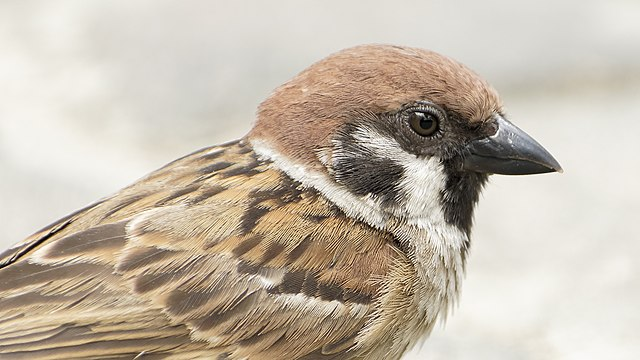
\includegraphics[width=.45\textwidth]{Passer_montanus_malaccensis}
    \caption{
      Eurasian tree sparrow (\textit{Passer montanus malaccensis}), adult
      male, in Kuala Lumpur, Malaysia. Taken on 31 January 2019, 15:20:47 by
      \href{
        https://commons.wikimedia.org/wiki/File:Passer_montanus_malaccensis_@_Kuala_Lumpur,_Malaysia_(1).jpg
      }{Peter P. Othagoer, Wikimedia Commons, CC BY 4.0}. \label{fig:sparrow}
    }
  \end{figure}
\end{frame}

\begin{frame}{\insertsubsectionhead}{Side-by-Side}
  The same as before, but the second image has been flipped horizontally
  (Figure~\ref{fig:sparrow2}).

  \begin{figure}
    \centering
    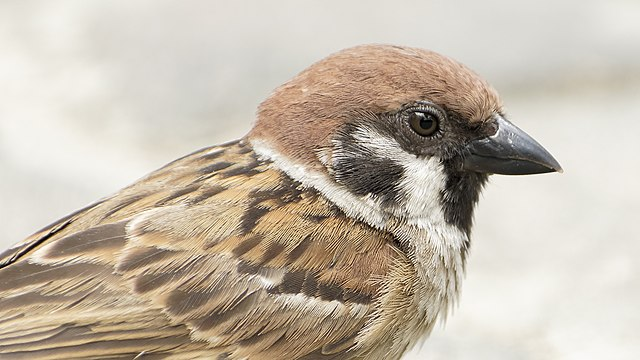
\includegraphics[width=.4\textwidth]{Passer_montanus_malaccensis}
    ~~~
    \reflectbox{
      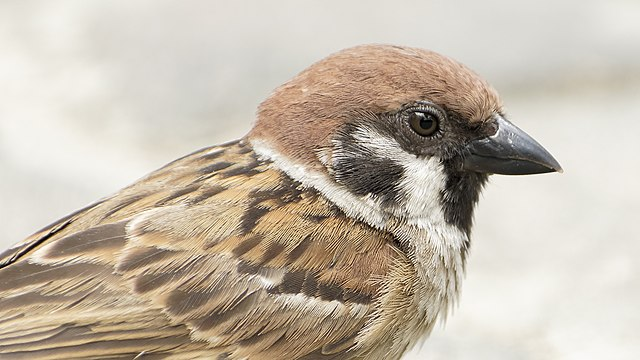
\includegraphics[width=.4\textwidth]{Passer_montanus_malaccensis}}
    \caption{Eurasian tree sparrow (\textit{Passer montanus malaccensis}),
      adult male, in Kuala Lumpur, Malaysia. Taken on 31 January 2019,
      15:20:47 by \href{
        https://commons.wikimedia.org/wiki/File:Passer_montanus_malaccensis_@_Kuala_Lumpur,_Malaysia_(1).jpg
      }{Peter P. Othagoer, Wikimedia Commons, CC BY 4.0}. \label{fig:sparrow2}
    }
  \end{figure}
\end{frame}

%%%%%%%%%%%%%%%%%%%%%%%%%%%%%%%%%%%%%%%%%%%%%%%%%
\subsection{Tables}
\begin{frame}{\insertsubsectionhead}
  An example table (Table~\ref{tab:norm}).

  \begin{table}
    \caption{A table containing data from the sample long table by
      \href{
        https://www.overleaf.com/latex/examples/a-longtable-example/xxwzfxkxxjmc
      }{LianTze Lim, Overleaf, CC BY 4.0}. \label{tab:norm}
    }
    \footnotesize
    \begin{center}
      \begin{tabular}{lll}
        \toprule
        \textbf{First column} & \textbf{Second column} &
        \textbf{Third column} \\
        \midrule
        One & abcdef ghjijklmn & 123.456778 \\
        One & abcdef ghjijklmn & 123.456778 \\
        One & abcdef ghjijklmn & 123.456778 \\
        One & abcdef ghjijklmn & 123.456778 \\
        One & abcdef ghjijklmn & 123.456778 \\
        \bottomrule
      \end{tabular}
    \end{center}
  \end{table}
\end{frame}

%%%%%%%%%%%%%%%%%%%%%%%%%%%%%%%%%%%%%%%%%%%%%%%%%
\subsection{Mathematics and Equations}
\begin{frame}{\insertsubsectionhead}
  Here's an example inline equation: \(\textrm{e}^{i\pi} + 1 = 0\). Some
  example equations are shown in Equation~\ref{eqn:int},
  Equation~\ref{eqn:trig}, and Equation~\ref{eqn:id}.

  \begin{equation}
    \label{eqn:int}
    \int x^n\,\mathrm{d}x = \frac{1}{n + 1}x^{n + 1}, \qquad n \neq -1
  \end{equation}

  \begin{equation}
    \label{eqn:trig}
    \sin \frac{\beta}{2} = \sqrt{\frac{1 - \cos \beta}{2}}
  \end{equation}

  \begin{equation}
    \label{eqn:id}
    \begin{bmatrix}
      n + 1 \\
      m + 1
    \end{bmatrix}
    = \sum_k
    \begin{pmatrix}
      n \\
      k
    \end{pmatrix}
    \begin{bmatrix}
      k \\
      m
    \end{bmatrix}
    = \sum^n_{k = 0}
    \begin{bmatrix}
      k \\
      m
    \end{bmatrix}
    (m + 1)^{n -k}
  \end{equation}
\end{frame}

%%%%%%%%%%%%%%%%%%%%%%%%%%%%%%%%%%%%%%%%%%%%%%%%%
\subsection{Code Blocks}
\begin{frame}[fragile,allowframebreaks]{\insertsubsectionhead}
% all indentation, line breaks, and spaces will be shown in output
% as it is verbatim code
% must use fragile for verbatim code
\begin{exampleblock}{Python}
% using custom style (py) defined in template
\begin{lstlisting}[style=py]
import os
import errno
# create directory if it doesn't already exist
fpath = 'data/'
try:
    os.makedirs(fpath)
except OSError as exception:
    if exception.errno != errno.EEXIST:
        raise
    else:
        print('\nBE CAREFUL! Directory %s already exists.' % fpath)
\end{lstlisting}
\end{exampleblock}

\begin{exampleblock}{Shell}
% using custom style (sh) defined in template
\begin{lstlisting}[style=sh]
#!/bin/sh

# change to home directory
cd $HOME

# delete all lines containing string in file
grep -v "string to delete" file.txt > tempfile.txt

# rename file
mv tempfile.txt file.txt
\end{lstlisting}
\end{exampleblock}
\end{frame}

%%%%%%%%%%%%%%%%%%%%%%%%%%%%%%%%%%%%%%%%%%%%%%%%%
\appendix

%%%%%%%%%%%%%%%%%%%%%%%%%%%%%%%%%%%%%%%%%%%%%%%%%
% Thank you slide
\begin{frame}
  \textbf{\LARGE Thank you for your attention!}

  % manual spacing between lines
  \vspace{16pt}
  % optional - copyright info
  % use \the\year\ to display the current year
  Copyright (c) \the\year\ Euclid of Alexandria
  \href{mailto:euclid@alexandria.edu}{\texttt{<euclid@alexandria.edu>}}.

  \vspace{8pt}
  % creative commons logo via fontawesome5
  {\Huge\faCreativeCommons\ \faCreativeCommonsBy}

  % license info
  Except where otherwise noted, the contents of this presentation are licensed
  under a Creative Commons Attribution 4.0 International license (CC BY 4.0)
  \href{https://creativecommons.org/licenses/by/4.0/}
  {\texttt{<creativecommons.org/licenses/by/4.0>}}.
\end{frame}

%%%%%%%%%%%%%%%%%%%%%%%%%%%%%%%%%%%%%%%%%%%%%%%%%
\section{References}
\begin{frame}[allowframebreaks]{\insertsectionhead}
  % references that have been cited in-text
  \references

  % references from the \nocite command
  \textbf{Further Reading}
  \furtherreading
\end{frame}

%%%%%%%%%%%%%%%%%%%%%%%%%%%%%%%%%%%%%%%%%%%%%%%%%
\end{document}
